%%%%%%%%%%%%%%%%%%%%%%%%%%%%%%%%%%%%%%%%%
% Beamer Presentation
% LaTeX Template
% Version 1.0 (10/11/12)
%
% This template has been downloaded from:
% http://www.LaTeXTemplates.com
%
% License:
% CC BY-NC-SA 3.0 (http://creativecommons.org/licenses/by-nc-sa/3.0/)
%
%%%%%%%%%%%%%%%%%%%%%%%%%%%%%%%%%%%%%%%%%

%----------------------------------------------------------------------------------------
%	PACKAGES AND THEMES
%----------------------------------------------------------------------------------------

\documentclass[aspectratio=169]{beamer}
\usepackage[utf8]{inputenc}
\usepackage{booktabs}
\usepackage{graphicx}
\usepackage{array}
\usepackage{caption}
\usepackage{threeparttable}
\usepackage{lscape}
\usepackage{import}
\usepackage{amsmath}
\usepackage{csvsimple}
\usepackage{siunitx}
\usepackage{subfigure}
\usepackage{filecontents}
\newenvironment{wideitemize}{\itemize\addtolength{\itemsep}{10pt}}{\enditemize}
\usepackage{appendixnumberbeamer}
\usepackage{float}
\usepackage{amsmath}  
\usepackage{tikz,pgfplots}
\usepackage{tkz-fct}
\usepackage{amsthm}
\pgfplotsset{compat=1.10}
\usepgfplotslibrary{fillbetween}
\newcommand{\vertLineFromPoint}[1]{
  \draw[dashed] 
  (#1) -- (#1|-{rel axis cs:0,0})
}
\newcommand{\horLineFromPoint}[1]{
  \draw[dashed] 
  (#1) -- (#1-|{rel axis cs:0,0})
}
\mode<presentation> {
\AtBeginSection[]
{
    \begin{frame}
        \frametitle{Table of Contents}
        \tableofcontents[currentsection]
    \end{frame}
}
% The Beamer class comes with a number of default slide themes
% which change the colors and layouts of slides. Below this is a list
% of all the themes, uncomment each in turn to see what they look like.

%\usetheme{default}
%\usetheme{AnnArbor}
%\usetheme{Antibes} -
%\usetheme{Bergen}
%\usetheme{Berkeley}
%\usetheme{Berlin}
\usetheme{Boadilla}
%\usetheme{CambridgeUS}
%\usetheme{Copenhagen} -
%\usetheme{Darmstadt}
%\usetheme{Dresden}
%\usetheme{Frankfurt}
%\usetheme{Goettingen}
%\usetheme{Hannover}
%\usetheme{Ilmenau}
%\usetheme{JuanLesPins}
%\usetheme{Luebeck}
%\usetheme{Madrid}
%\usetheme{Malmoe}
%\usetheme{Marburg}
%\usetheme{Montpellier}
%\usetheme{PaloAlto}
%\usetheme{Pittsburgh}
%\usetheme{Rochester} -
%\usetheme{Singapore}
%\usetheme{Szeged}
%\usetheme{Warsaw}

% As well as themes, the Beamer class has a number of color themes
% for any slide theme. Uncomment each of these in turn to see how it
% changes the colors of your current slide theme.

%\usecolortheme{albatross}
%\usecolortheme{beaver}
%\usecolortheme{beetle}
%\usecolortheme{crane}
%\usecolortheme{dolphin}
%\usecolortheme{dove}
%\usecolortheme{fly}
%\usecolortheme{lily}
%\usecolortheme{orchid}
%\usecolortheme{rose}
%\usecolortheme{seagull}
%\usecolortheme{seahorse}
%\usecolortheme{whale}
%\usecolortheme{wolverine}

%\setbeamertemplate{footline} % To remove the footer line in all slides uncomment this line
\setbeamertemplate{footline}[frame number] % To replace the footer line in all slides with a simple slide count uncomment this line
\setbeamertemplate{theorems}[numbered]
\setbeamertemplate{navigation symbols}{} % To remove the navigation symbols from the bottom of all slides uncomment this line
}
\setbeamertemplate{caption}{\raggedright\insertcaption\par}
  \setbeamertemplate{enumerate items}[default]
\usepackage{graphicx} % Allows including images
\usepackage{booktabs} % Allows the use of \toprule, \midrule and \bottomrule in tables
%\usepackage {tikz}
\newtheorem*{theorem*}{Theorem}
\newtheorem*{lemma*}{Lemma}
\newtheorem*{proposition}{Proposition}
\newtheorem*{corollary*}{Corollary}
\newtheorem*{definition*}{Definition}
\DeclareMathOperator*{\argmin}{arg\,min}
\newtheorem*{assumption}{Assumption}
\usetikzlibrary {positioning}
%\usepackage {xcolor}

%----------------------------------------------------------------------------------------
%	TITLE PAGE
%----------------------------------------------------------------------------------------

\title[Risk]{Lecture 2: Monopoly} % The short title appears at the bottom of every slide, the full title is only on the title page

\author{Jacob Kohlhepp} % Your name
\institute[UCLA] % Your institution as it will appear on the bottom of every slide, may be shorthand to save space
{
Econ 101 \\ % Your institution for the title page
\medskip
}
\date{\today} % Date, can be changed to a custom date

\begin{document}

\begin{frame}
\titlepage % Print the title page as the first slide
\end{frame}

\begin{frame}{Introduction}
\begin{wideitemize}
    \item In Econ 11, we assumed actors (firms, consumers, etc) took price as \textit{given.}
    \item Even when there were only two consumers in an endowment economy, we assumed price was taken as given.
    \item This is often not realistic. Sometimes buyers/sellers are so large they impact the price.
    \item When an entity has the ability to unilaterally influence price, we say it has ``market power."
    \item We will study three types of market power:
    \begin{enumerate}
        \item Monopoly: Maximum Market Power Supply Side (this lecture)
        \item Oligopoly: Intermediate Market Power Supply Side (in the future)
        \item Monopsony: Maximum Market power Demand Side (practice problems)
    \end{enumerate}
\end{wideitemize}

\end{frame}

\begin{frame}{Why Care About Monopolies?}
    \begin{columns}[T] % align columns
\begin{column}{.63\textwidth}
\begin{wideitemize}
        \item Many real life examples.
        \begin{enumerate}
            \item DeBeers Diamonds
            \item OPEC Oil (dynamic oligopoly resulting in static monopoly) 
            \item Utilities (government granted)
            \item Patents (vaccines, etc).
            \item Unique goods (collectibles, one-of-a-kind)
            \item Network goods: Facebook, dating apps, Google
        \end{enumerate}
        \item The government has long tried to stop them.
        \begin{enumerate}
            \item Teddy Roosevelt Trust busting back in 1899
            \item Merger reviews by DOJ today.
            \item Congressional hearings on big tech.
        \end{enumerate}
        \item They can greatly reduce consumer surplus.
\end{wideitemize}
\end{column}%
\hfill%
\begin{column}{.34\textwidth}
\resizebox{\textwidth}{!}{
  \includegraphics{cartoon-Theodore-Roosevelt-trust-buster-e1560544846616.jpg}
  
}
\end{column}%
\end{columns}

  \hfill Source: Lloyd Constantine
\end{frame}

\begin{frame}{Thought Exercise}
    \begin{wideitemize}
            \item Question: How many firms do we need for perfect competition? Answer in the poll.
            \pause \item Surprisingly, we only need 1.
            \pause\item Why? We can have one firm selling at price equal to marginal cost and an infinite number of firms ready to jump in if the firm sets price above marginal cost.
            \pause\item \textbf{Big Takeaway:} Just like every square is a rectangle but not every rectangle is a square, monopolies always have one firm but not all situations with one firm are monopolies.
            \pause\item There needs to be something stopping the firms from entering.
            \pause\item The technical term for these: \textbf{entry barriers}.
    \end{wideitemize}
\end{frame}

\begin{frame}{Entry Barriers}

\begin{wideitemize}
        \item Legal barriers (patents)
        \item Political barriers (lobbying, secrecy, access to unique resources)
        \item Technical barriers (knowledge of production techniques, increasing returns to scale)
        \item Others?
\end{wideitemize}
    
\end{frame}

\begin{frame}{Notation, Terms, Definitions}
In this class:
    \begin{wideitemize}
            \item $q$ is total market quantity.
            \item $c(q)$ is the cost function.
            \item $d(p)$ is the demand function given the price.
            \item $p(q)$ is the inverse demand function: it comes from inverting $d(p)$ so that we have price in terms of quantity.
    \end{wideitemize}
\end{frame}

\begin{frame}{The Monopoly Model}
\begin{wideitemize}
        \item One firm (monopolist) which can choose quantity $q$ to produce.
        \item Cost is given by $c(q)$.
        \item The firm faces an inverse demand function $p(q)$ (derived from aggregate demand function).
        \item The firm maximizes profit:
        \[\max_q \pi = q\cdot p(q) - c(q) \]
        \item Notice this is just revenue less cost like in Econ 11.
        \end{wideitemize}
\end{frame}

\begin{frame}{Solve The Model}
    \begin{wideitemize}
            \item Like in Econ 11, $MC=MR$. Or just take FOC:
            \[\frac{\partial \pi}{\partial q} = p(q) +q\cdot p'(q) - c'(q) =0 \leftrightarrow \]
            \item The last equation is just $MR=MC$!
            \item $q_{MON}$ which solves the last equation is the monopoly quanity.
            \item Monopoly price is $p(q_{MON})$.
    \end{wideitemize}
\end{frame}

\begin{frame}{Notes About the Monopoly Solution}
\begin{wideitemize}
        \item  The first-order condition:
     \[\frac{\partial \pi}{\partial q} = p(q) +q\cdot p'(q) - c'(q) =0\]
     is the \textbf{general solution} to the problem.
     \item If we are given a specific cost function and inverse demand we can plug in to get the solution.
    
\end{wideitemize}
   
\end{frame}

\begin{frame}{Comparing to Perfect Competition}
\begin{wideitemize}
        \item In perfect competition, producers take price as given. That is, they assume that their quantity cannot impact price.
        \item In our model, this is equivalent to producers thinking $p'(q)=0$. 
        \item This feels weird because price does depend on quantity. We can rationalize this by saying that under perfect competition there are many firms whose totla output equals $q$. Any individual firm cannot shift price by adjusting quantity.
        \item Therefore we can think of perfect competition using our monopoly model!
        \item If we plug in $p'(q)=0$, to the FOC:
        \[\frac{\partial \pi}{\partial q} = p(q) -c'(q)=0 \leftrightarrow p(q) = c'(q)\]
        \item We find the result from Econ 11: under perfect competition producers set price equal to marginal cost!
\end{wideitemize}
\end{frame}

\begin{frame}{Graphical Comparison of Perfect Competition and Monopoly}
    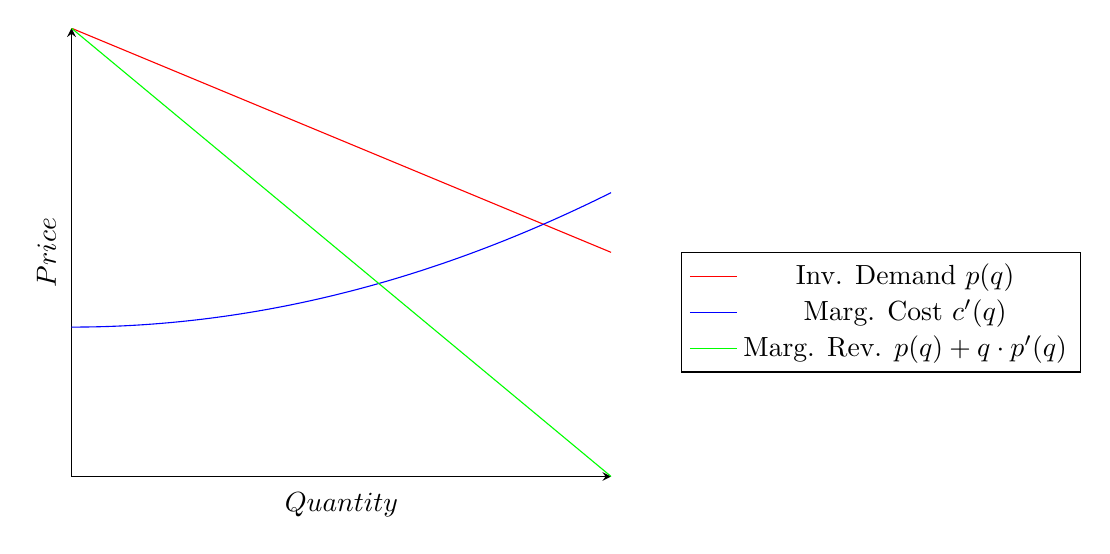
\begin{tikzpicture}
\begin{axis}[
    axis lines = left,
    xlabel = \(Quantity\),
    ylabel = {\(Price\)},
    ytick=\empty,
    xtick=\empty,
    legend  style={at={(1.50 ,0.5)},
    anchor=north,legend  columns =1},
]

%Below the red parabola is defined
\addplot [
    domain=0:6, 
    samples=100, 
    color=red,
    name path=d
]
{8-x};
\addlegendentry{\(\text{Inv. Demand } p(q)\)}
%Here the blue parabola is defined
\addplot [
    domain=0:6, 
    samples=100, 
    color=blue,
    name path=mc
    ]
    {0.1*x^2};
\addlegendentry{\(\text{Marg. Cost } c'(q)\)}
\addplot [
    domain=0:6, 
    samples=100, 
    color=green, 
    name path=mr
    ]
    {8-2*x};
\addlegendentry{\(\text{Marg. Rev. } p(q)+q\cdot p'(q)\)}
\end{axis}
\end{tikzpicture}

From the picture we see that $q_{mon}<q_{perfect}$. It turns out this is true in many cases!
\end{frame}


\begin{frame}{Linear Inverse Demand, Quadratic Costs}
Suppose $c(q)=x^2$ and $p(q)=2-3q$. What is the monopolist quantity and price? What is the perfect competition quantity and price?

\vspace{5mm}

See handwritten notes for solution.

\end{frame}


\begin{frame}{Deriving Linear Demand}

\begin{wideitemize}
        \item So far, we have assumed inverse demand is given.
        \item But where does inverse demand come from?
        \item We will go through deriving it for uniform willingness to pay.
        \item A good exercise is to solve when inverse demand takes different forms. See recommended problem set.
        
\end{wideitemize}
\end{frame}

\begin{frame}{Deriving Linear Demand}
\begin{wideitemize}
        \item Fix the number of consumers in the economy to be 1.
        \item Each consumer has a different willingness to pay given by $W$.
        \item Now we say that the ``amount" (technical term: density) of consumers with willginess to pay $w$ is given by some function $f(w)$.
        \item A consumer buys if $W\geq p$.
        \item To get demand we need to ``sum up" the consumers which buy. because we have infinite consumers (a continuum of consumers) summing up means integrating:
        
        \[d(p) = \int^{\infty}_p f(w)dw\]
\end{wideitemize}
\end{frame}

\begin{frame}{Deriving Linear Demand}
\begin{wideitemize}
        \item Suppose willingness to pay has density:
        \[f(w) = \begin{cases} \frac{1}{b-a} \text{ if } a\leq w\leq b\\
        0 \text{ else } \end{cases}\]
        \item So maximum willingness is $b$, minimum $a$, and people are evenly distributed in between.
        \item Then the demand for a price that is $a \leq p \leq b$: (fill in) \pause
        \[d(p)=\int^{\infty}_p f(w) dw= \int^{\infty}_b 0 dw + \int^{b}_p\frac{1}{b-a}  dw =\frac{b-p}{b-a} = \frac{b}{b-a} - \frac{1}{b-a}\cdot p  \]
        \item So we get \textbf{linear demand}! If $b=1, a=0$:
        \[d(p)=1-p\]
    
\end{wideitemize}
\end{frame}

\begin{frame}{Deriving Linear Inverse Demand}
To get inverse demand, we set $d(p)$ from the last page equal to $q$ (quantity). Then solve for $p$. (fill in) \pause 
\[d(p)= \frac{b}{b-a} - \frac{1}{b-a}\cdot p =q \]
\[b - (b-a)q =p(q) \]
\end{frame}


\begin{frame}{Big Ideas/Intuition}
\begin{wideitemize}
        \item We know now that under monopoly, quantity supplied is lower than under perfect competition.
        \item The reason is that the monopolist can keep the price artificially high and not worry about being undercut by competitors. 
        \item This is market power: one firm controls an entire side of the market.
        \item Note that this is \textbf{not} the same as a firm being able to ``charge whatever it wants." The monopolist is still constrained by the law of demand: higher prices means less customers.
\end{wideitemize}
\end{frame}

\begin{frame}{Welfare Analysis}
\begin{wideitemize}
        \item We want to understand how the presence of a monopolist impacts welfare.
        \item First, recall the idea of consumer surplus:
        \begin{definition}
            \textbf{Consumer surplus} is the amount of money a consumer would pay to make a transaction at a given price.
        \end{definition}
        \item Total consumer surplus is the area below the demand curve and above the price, and can be calculated as:
        \[CS(q) = \int^q_0 p(x) - p(q)dx \]
\end{wideitemize}
    
\end{frame}
\begin{frame}{Welfare Analysis}
\begin{wideitemize}
        \item Now consider producer surplus. This is captured by profits, which are given by:
        \[\Pi(q) = p(q) q - c(q)\]
        \item Total surplus is the sum of producer surplus and consumer surplus:
        \[TS(q) = CS(q)+\Pi(q) = \int^q_0 p(x) - p(q)dx+p(q) q - c(q)\  \]
        \item Using the Fundamental Theorem of Calculus we can re-write this as:
        \[TS(q) = \int^q_0 p(x) dx- c(q)  \]
\end{wideitemize}
    
\end{frame}

\begin{frame}{Welfare Analysis}
Question: If a social planner could choose $q$ to maximize total surplus, what would they choose?
Answer: Just solve the below equation.
\[TS = \max_q \int^q_0 p(x) dx- c(q)\]
FOC: 

\[\frac{\partial TS}{\partial q} = p(q)-c'(q)=0\]

This should look familiar! It is exactly the $MC=p$ from perfect competition.

\vspace{5mm}

\textbf{Big Idea:} Perfect Competition maximizes total surplus, and monopoly does not. There will always be welfare loss from monopoly.

\end{frame}

\begin{frame}{Deadweight Loss}
    \begin{definition}
    \textbf{Deadweight loss} is the difference between total surplus under the social planner's optimum and the actual situation.
    \end{definition}
    \begin{wideitemize}
            \item The social planner's optimum is the competitive outcome.
            \item Therefore dead weight loss under monopoly is perfect competition total surplus minus monopoly total surplus:
            \[DWL = TS(q_{perfect})-TS(q_{mon})\]
            \item We can interpret this as the value of the transactions that are foregone under monopoly.
            \item Individuals with willingness to pay between $p_{mon}$ and $p_{perfect}$ are not buying under monopoly but are buying under perfect competition.
            
    \end{wideitemize}
\end{frame}

\begin{frame}{Graphing Deadweight Loss}
\centering
    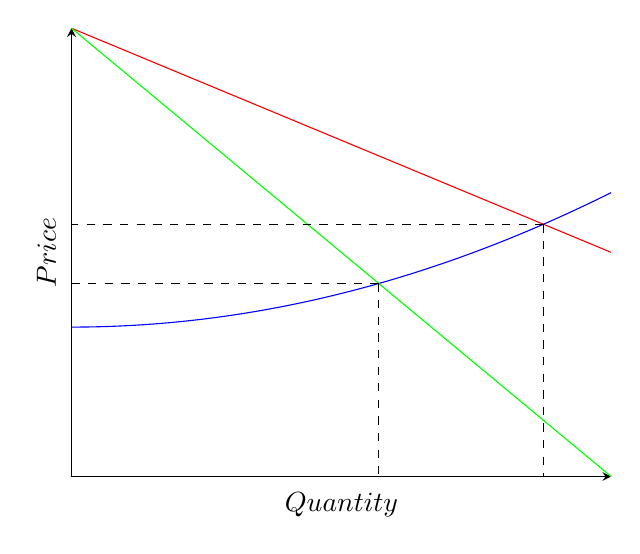
\begin{tikzpicture}
\begin{axis}[
    axis lines = left,
    xlabel = \(Quantity\),
    ylabel = {\(Price\)},
    ytick=\empty,
    xtick=\empty
]

%Below the red parabola is defined
\addplot [
    domain=0:6, 
    samples=100, 
    color=red,
    name path=d
]
{8-x};
%Here the blue parabola is defined
\addplot [
    domain=0:6, 
    samples=100, 
    color=blue,
    name path=mc
    ]
    {0.1*x^2};
\addplot [
    domain=0:6, 
    samples=100, 
    color=green, 
    name path=mr
    ]
    {8-2*x};
 \path [name intersections={of=mc and d, by={x1}}];
 \path [name intersections={of=mr and mc, by={x2}}];
 \vertLineFromPoint{x1};
\horLineFromPoint{x1};
 \vertLineFromPoint{x2};
\horLineFromPoint{x2};
 \end{axis}
\end{tikzpicture}
\end{frame}

\begin{frame}{Monopsony}
\begin{wideitemize}
        \item So far we have considered when a single entity has all market power on the supply side.
        \item But what if a single entity has all market power on the demand side?
        \item This is called \textbf{monopsony.}
        \item Examples:
        \begin{enumerate}
            \item Large employers in small towns.
            \item Large producers of a final good buying inputs.
        \end{enumerate}
        \item Our analysis so far basically applies identically to monopsony.
        \item We will now use our monopoly/monosony model to think about minimum wages.
\end{wideitemize}
    
\end{frame}

\begin{frame}{Application: Monopsony and the Minimum Wage}{Background}

\begin{wideitemize}
        \item Prior to Card and Krueger (1993), many economists believed minimum wages should reduce labor demand.
        \item Why? Because if labor markets are like any other market in perfect competition, the law of demand says that a higher price must mean less demand.
        \item But a series of studies have found mixed results: sometimes binding minimum wages seem to have no impact or a slight positive impact on employment (quantity in the language of our model).
        \item But why? A leading argument: because employers have market power, and are buying labor at a price below the competitive price.
\end{wideitemize}
\end{frame}

\begin{frame}{Application: Monopsony and the Minimum Wage}{A Simple Model}
\begin{wideitemize}
        \item Consider a local labor market, where Walmart is a monopsonist of low-skill labor.
        \item Using a unit of labor Walmart produces $F(q)$ units of revenue.
        \item Walmart selects a quantity of labor, call it $q$, knowing that it is the only buyer and can thus impact the wage $w$.
        \item A large number of people in the town supply labor according to labor supply function $l(w)$.
        \item This induces inverse labor supply function $w(q)$ (aka the market-clearing wage function).
\end{wideitemize}
\end{frame}


\begin{frame}{Application: Monopsony and the Minimum Wage}{Monopsony Equilibrium}
 Walmart solves:
        \[\max_q F(q) - w(q)\cdot q \]
which gives FOC:
\[F'(q)-w'(q)q-w(q)=0\]
Suppose $F(q)=log(q)+20$, $w(q)=2q$:
\[q^{-1} - 2q-2q=0 \implies 2q^2-4q=0 \implies q_{mon} =0.5\]
\[w_{mon} =1 \]
\end{frame}


\begin{frame}{Application: Monopsony and the Minimum Wage}{Perfectly Competitive Equilibrium}
Under a competitive labor market, we have that wages are taken as given. Then $q_{perfect}$ solves:
\[F'(q)-w(q)=0\]
\[q^{-1} - 2q=0 \implies 1-2q^2=0 \implies q_{perfect} \approx 0.707  \]
\[w_{perfect} \approx 1.414 \]
Thus labor is under supplied and demanded under monopsony. The wage is also lower.
 \end{frame}
 
\begin{frame}{Application: Monopsony and the Minimum Wage}{Government Imposes Minimum Wage of $\bar w$}
        \[\max_q log(q) - 2q^2 +20 \qquad \text{ s.t. } q\geq \bar w/2 \]
\begin{wideitemize}
          \item If $q> 3.25$ profit becomes negative. So if $\bar w/2 > 3.25 \implies \bar w > 6.5$ Walmart exits.
          \item  If $6.5\geq \bar w \geq 1$ the minimum wage is above the monopsonist wage so profit is decreasing in the wage. Thus the min. wage binds and $w = \bar w$ so $q=\bar w/2$.
          \item If $\bar w<1$ the min. wage does not bind, then the monopsonist sets the wage at $w_{mon}$.
        \item In summary, labor demand under the min. wage is:
        \[q_{minwage} = \begin{cases} 0 \text{ if } \bar w > 6.5\\
        \bar w/2 \text{ if }  6.5\geq \bar w \geq 1\\
        0.5 \text{ else }\end{cases}\]

\end{wideitemize}

  \end{frame}
\begin{frame}{Application: Monopsony and the Minimum Wage}{Graphing the Minimum Wage}

 
    \end{frame}
    
\begin{frame}{Application: Monopsony and the Minimum Wage}{Discussion}
\begin{wideitemize}
        \item The bottomline: in a labor market characterized by extreme market power (monopsony) minimum wages can increase employment.
        \item If the minimum wage is set too high, it can cause market exit.
        \item How do we know if there is market power?
        \item Optimal minimum wage is of course to set $\bar w=w_{perfect}$.
        \item But doing this requires knowing the true competitive wage.
        \item \textbf{Discussion:} Given this, do you think a $\$15$ national minimum wage is appropriate?
\end{wideitemize}
\end{frame}
\end{document}

